\documentclass[a4paper]{article}
\usepackage[spanish]{babel}
\usepackage[utf8]{inputenc}
\usepackage{graphicx}
\usepackage{enumerate}
\usepackage{listings}
\usepackage{color}
\usepackage{indentfirst}
\usepackage{fancyhdr}
\usepackage{latexsym}
\usepackage[colorlinks=true, linkcolor=black]{hyperref}
%\usepackage{makeidx}
%\usepackage{float}
\usepackage{wrapfig}
\usepackage{calc}
\usepackage{amsmath, amsthm, amssymb}
\usepackage{amsfonts}
%\lstset{language=C}
\definecolor{gray}{gray}{0.5}
\definecolor{light-gray}{gray}{0.95}
\definecolor{orange}{rgb}{1,0.5,0}

\usepackage{fancyhdr}
\pagestyle{fancy}

%\renewcommand{\chaptermark}[1]{\markboth{#1}{}}
\renewcommand{\sectionmark}[1]{\markright{\thesection\ - #1}}

\fancyhf{}

\fancyhead[LO]{Sección \rightmark} % \thesection\ 
\fancyfoot[LO]{\small{Yanet Giuseppin, Laura Muiño, Javier San Miguel, Axel Straminsky}}
\fancyfoot[RO]{\thepage}
\renewcommand{\headrulewidth}{0.5pt}
\renewcommand{\footrulewidth}{0.5pt}
\setlength{\hoffset}{-0.8in}
\setlength{\textwidth}{16cm}
%\setlength{\hoffset}{-1.1cm}
%\setlength{\textwidth}{16cm}
\setlength{\headsep}{0.5cm}
\setlength{\textheight}{25cm}
\setlength{\voffset}{-0.7in}
\setlength{\headwidth}{\textwidth}
\setlength{\headheight}{13.1pt}

\renewcommand{\baselinestretch}{1.1}  % line spacing


% \setcounter{secnumdepth}{2}
\usepackage{underscore}
\usepackage{caratula}
\usepackage{url}
\usepackage{float}
\usepackage{algorithm}
\usepackage[noend]{algpseudocode}





\newcommand{\cod}[1]{{\tt #1}}
\newcommand{\negro}[1]{{\bf #1}}
\newcommand{\ital}[1]{{\em #1}}
\newcommand{\may}[1]{{\sc #1}}
\newcommand{\tab}{\hspace*{2em}}

\hypersetup{
 pdfstartview= {FitH \hypercalcbp{\paperheight-\topmargin-1in-\headheight}},
 pdfauthor={Grupo},
 pdfsubject={Dise\~{n}o}
}

\lstdefinestyle{customc}{
  backgroundcolor=\color{light-gray},
  belowcaptionskip=1\baselineskip,
  breaklines=true,
  numbers=left,
  xleftmargin=\parindent,
  language=C,
  showstringspaces=false,
  basicstyle=\footnotesize\ttfamily,
  keywordstyle=\bfseries\color{blue},
  commentstyle=\itshape\color{gray},
  identifierstyle=\color{black},
  stringstyle=\color{orange},
}

\lstdefinestyle{customasm}{
  backgroundcolor=\color{light-gray},
  belowcaptionskip=1\baselineskip,
  numbers=left,
  xleftmargin=\parindent,
  language=[x86masm]Assembler,
  keywordstyle=\bfseries\color{blue},
  basicstyle=\footnotesize\ttfamily,
  commentstyle=\itshape\color{gray},
}

\lstset{escapechar=@}


\begin{document}

\thispagestyle{empty}
\materia{Métodos Numéricos}
\submateria{Segundo Cuatrimestre de 2015}
\titulo{Trabajo Práctico II}
%\subtitulo{Scheduling}
\integrante{Yanet Giuseppin}{184/11}{yanetagiu@yahoo.com}
\integrante{Laura Muiño}{399/11}{mmuino@dc.uba.ar}
\integrante{Javier San Miguel}{786/10}{javiersm00@gmail.com}
\integrante{Axel Straminsky}{769/11}{axelstraminsky@gmail.com}

\makeatletter

\maketitle
\newpage

\thispagestyle{empty}
\vfill

\thispagestyle{empty}
\vspace{3cm}
\tableofcontents
\newpage

\newenvironment{myindentpar}[1]
{\begin{list}{1}
         {\setlength{\leftmargin}{#1}}
         \item[]
}
{\end{list} }

%\normalsize
\newpage


%\section{Introducción}

Queremos resolver el problema de los rankings de las páginas web, de manera que la búsqueda de una página sea mas eficiente y a la vez que devuelva mejores resultados. \\

Vamos a utilizar dos métodos para este propósito. Cada uno de ellos tiene un criterio diferente para ordenar las páginas. \\

El primero se denomina $PageRank$. Es la primera versión del algoritmo que usó Google para posicionarse por encima de los otros buscadores en sus inicios. Usa propiedades de álgebra lineal y de matrices que vamos a anunciar en el trabajo y explicar en la medida que se necesite.\\

El segundo se denomina $IN-DEG$ y es mas sencillo, ya que sólo utiliza la cantidad de links entrantes de las páginas para definir el ranking.\\

El algoritmo de PageRank es mas complejo: Le asigna a cada página un puntaje que depende no solamente dqe la cantidad de links entrantes, sino de la importancia que tiene cada link, que depende del puntaje de la página de origen y de los links salientes de ella. Otro factor que afecta el ranking es la probabilidad de que el navegante salte a una página sin usar link. \\

De esta manera se evita que una página que es apuntada por muchas otras poco importantes, tenga mayor puntaje que otra que tiene menos links entrantes, pero que es apuntada por páginas más importantes. Este es un caso en que el algoritmo de $IN-DEG$ no da buenos resultados pero el $PageRank$ si.
%Veamos un ejemplo de esto, y los resultados de ambos algoritmos:\\


%Imagen de grafo de paginas 1
\begin{wrapfigure}{r}{0.6\textwidth}
  \vspace{-20pt}
  \begin{center}
    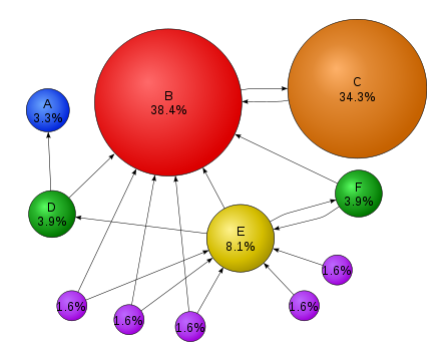
\includegraphics[scale= 0.6]{imagenes/ejemplo-grafo-1.png}
  \end{center}
  \vspace{-20pt}
   \caption[Caption for LOF]{El algebra lineal detrás de los buscadores de internet. Carlos D'Andrea.\footnotemark}
  \vspace{-10pt}
  \label{fig:img1}
\end{wrapfigure}



%Lectura: https://atlas.mat.ub.edu/personals/dandrea/2012_09_25_escrito_google.pdf \\
\footnotetext{Lectura: https://atlas.mat.ub.edu/personals/dandrea/2012_09_25_escrito_google.pdf.}

En el grafo de la figura \ref{fig:img1}, los nodos son páginas web y los ejes son los links. Los porcentajes muestran el orden en el ranking según el algoritmo de $PageRank$. La primera página es la B, luego la C, etc.\\

 Si aplicaramos el algoritmo de $IN-DEG$, la primera página tambien resultaría ser la B, pero la segunda la E. Y la C, que tiene un link entrante de la página que parece ser más importante (B), estaría en último lugar. Por eso en este caso es más justo el algoritmo de $PageRank$.\\

Para este trabajo implementamos ambos algoritmos y analizamos los resultados obtenidos en diferentes escenarios.\\

También realizamos mejoras para el tiempo de ejecución y el espacio usado por el algoritmo de $PageRank$. Una forma de lograr esto es utilizar estructuras de datos que aprovechen ciertas condiciones que suelen darse en la realidad.\\

 Las optimizaciones que se hacen para reducir el tiempo y espacio de este algoritmo son importantes, porque es realidad es usado para procesar muy grandes cantidades de información y generar rankings de millones de páginas web. Haremos entonces un análisis temporal y espacial.\\

Por otro lado, hicimos una leve modificación al algoritmo de $PageRank$ para determinar rankings de equipos en una liga deportiva. \\

En $PageRank$ se representa a las páginas web como los nodos de un grafo en el que los ejes son los links. De la misma manera se puede representar a los equipos de una liga como los nodos y los resultados de los partidos como los ejes con un cierto peso, para determinar un ranking.\\

Como los grafos de las ligas no son tan grandes como los de las webs, no nos interesa analizar los aspectos mas computacionales del algoritmo, como tiempo y memoria. Vamos a analizar los diferentes resultados que obtuvimos con este algoritmo para ciertos deportes, y vamos a comparar nuestros resultados con los resultados de los métodos estándar.\\


% imagen grafo4equipos
\begin{wrapfigure}{r}{0.5\textwidth}
  \vspace{-20pt}
  \begin{center}
    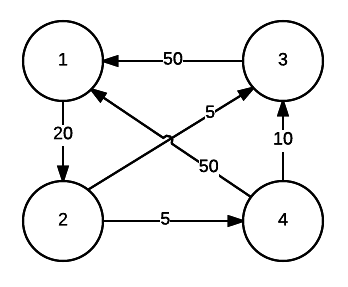
\includegraphics[scale= 0.8]{imagenes/grafo4equipos.png}
  \end{center}
  \vspace{-20pt}
  \caption{Mensaje a completar.}
  \vspace{-10pt}
  \label{fig:img2}
\end{wrapfigure}


El grafo de la figura \ref{fig:img2} representa los partidos de una liga de algun deporte. Son 4 equipos (los nodos) y todos juegan contra los otros 3. Las aristas son la diferencia de puntos del partido entre los 2 equipos. Los nodos de llegada de las aristas son los equipos ganadores.\\

Una alternativa para generar el ranking sería ordenarlos por cantidad de partidos ganados, y en caso de empate ordenarlos por puntos a favor. El ranking dejaría en primer lugar al equipo 1, en segundo lugar al equipo 3, en tercer lugar al equipo 2 y el último lugar el 4.\\

En cambio si usaramos el algoritmo de $PageRank$ para obtener el ranking, quedaría el equipo 1 en primer lugar también, pero en segundo lugar el equipo 2 y en tercero el 3. Esto es porque también importa a quien le ganó cada equipo, y el equipo 2 le ganó al 1 que tiene más partidos ganados y muchos puntos a favor. Con este algoritmo entonces podemos generar rankings que dependan de más variables.\\







%\newpage

% \section{Desarrollo}

\subsection{PageRank}

El algoritmo PageRank genera un ranking de páginas web de acuerdo a la importancia de cada página, esto es utilizado por los buscadores Web para devolver el resultado más relacionado a la búsqueda realizada por el usuario.\\

<<<<<<< HEAD
Para determinar que página es la más importante, el algoritmo define el puntaje de cada página como la siguiente sumatoria:

\begin{eqnarray}
x_k = \sum_{j \in L_k} \frac{x_j}{n_j},~~~~k = 1,\dots,n.\label{eq:ecuacion1}
\end{eqnarray}

donde $x_{j}$ es la importancia de la página j, $n_{j}$ es la cantidad de links salientes de la página j y $L_{k}$ el conjunto de páginas web con links salientes a j. Dichos puntajes siempre son mayores o iguales a cero, con lo que el puntaje cero corresponde a la página menos importante.\\


Estas ecuaciones pueden ser escritas como un sistema $Ax = x$, con x el vector de los puntajes que buscamos, ya que cada puntaje se obtiene con los de sus páginas vecinas (o sea las del conjunto $L_{k}$).\\

Además, A es una matriz estocástica por columnas, veamos por qué vale esto. Por definición del sistema de ecuaciónes en \ref{eq:ecuacion1} vale que

\begin{equation*}
A_{ij} = \left\{
	\begin{array}{cl}
	\frac{1}{n_{j}} & \text{si hay un link de } j \text{ a } i,\\
	0 & \text{en caso contrario.}\\
	\end{array} \right.
\end{equation*}

Con lo cual, la j-ésima columna tiene $n_{j}$ elementos de valor $\frac{1}{n_{j}}$, cuya suma es uno. Con la siguiente proposición, obtenemos que una matriz estocástica por columnas tiene autovalor 1.\\

Proposición: Toda matriz estocástica por columna tiene a uno como autovalor.
Demostración: Sea $A \in R^{nxn}$ una matriz estocástica por columna y sea e $\in R^{n}$ un vector columna con todos sus elementos unos. Sabemos que A y $A^{T}$ tienen los mismos autovalores.
Como A es estocástica por columnas, vale que $A^{T} x e = e$ pues las columnas de A (y filas de $A^{T}$) suman uno. Luego como $\lambda = 1$ es autovalor de $A^{T}$ también lo es de A. \\

Luego el problema original equivale a encontrar el autovector x con autovalor 1 para la matriz cuadrada A, es decir, resolver el sistema $Ax = \lambda x$.

Sin embargo, se presentan dos problemas: no sabemos si el autovalor uno tiene multiplicidad uno (o sea, no sabemos si hay una única solución o multiples) y  hay problemas con aquellos nodos que no tengan salida (o sea, páginas web que no apuntan a ninguna otra, no tienen salida).\\



Para encontrar el autovalor de la matriz correspondiente al autovalor $\lambda$, aplicamos el algorítmo iterativo de la potencia.\\

Implementamos PageRank de la siguiente manera


\begin{algorithm}
\caption{Método de la Potencia}\label{metpot}
\begin{algorithmic}[1]

  \Function{MetodoPotencia}{Matriz A, vector x, double c, tolerance, maxIter}%\Comment{con $A \in R^{(nxm)*(nxm)}$, $b \in R^{nxm}$}

    \State $x = x/\lVert \mathbf{p} \rVert _{1}$
    \While{ no se alcance la iteracion máxima}
	    \State resuelvo sistema y = A.(1-c)*x + ms
 	    \State obtengo norma de y
 	    \State 	defino error como la norma uno de la resta entre x e y
      \If {difieren en menos del error tolerado}
      	\State devuelvo vector y con su norma como autovalor
      \Else
        \State x = y
      \EndIf
    \EndWhile
    \Return false
  \EndFunction

\end{algorithmic}
\end{algorithm}

% \newpage

% \section{Experimentación}

%Imagen 1
\begin{wrapfigure}{r}{0.6\textwidth}
  \vspace{-20pt}
  \begin{center}
    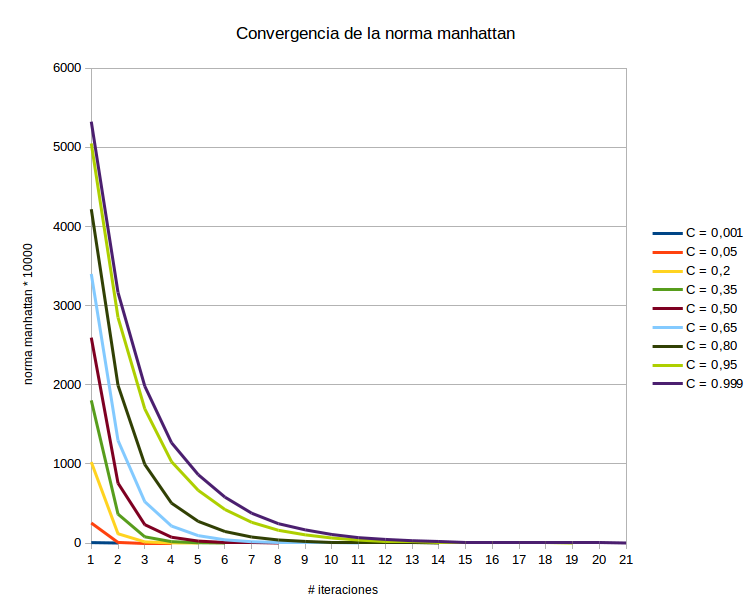
\includegraphics[scale= 0.6]{imagenes/convergencia1.png}
  \end{center}
  \vspace{-20pt}
   \caption{Con tantas páginas y tantos links.}
  \vspace{-10pt}
  \label{fig:img1}
\end{wrapfigure}

Para poder analizar la convergencia de PageRank realizamos mediciones de la cantidad de iteraciones que realiza el método de la potencia para el algoritmo, que termina cuando la norma de Manhattan es menor que un determinado valor muy cercano a 0.\\

Usamos tres instancias generadas al azar: La primera de 1000 páginas y 3000 links, la segunda de la misma cantidad de páginas pero 10000 links y la tercera de 500 páginas y 150000 links.\\

Nos interesa ver qué hace que el algoritmo termine en una menor cantidad de pasos y qué relación hay entre ese número y el valor de $c$. Ejecutamos $PageRank$ para cada instancia con una tolerancia fija de 0,00001, variando el valor del $c$ desde 0,001 hasta 0,999. Cada gráfico corresponde a los resultados obtenidos para una instancia distinta.\\



%Imagen 2
\begin{figure}[h]
  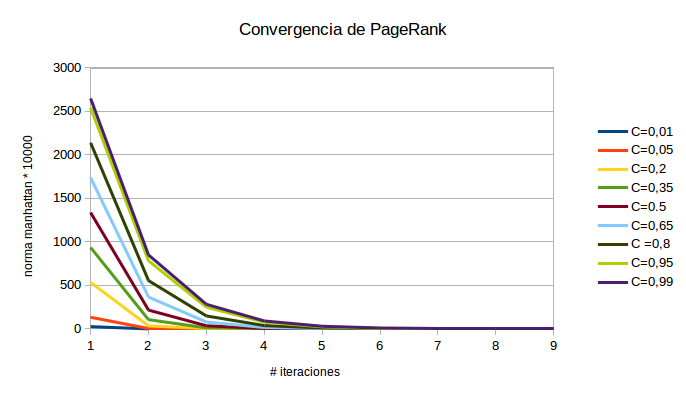
\includegraphics[scale= 0.6]{imagenes/convergencia2.png}
   \caption{Con tantas páginas y tantos links.}
  \label{fig:img1}
\end{figure}


\newpage

%Imagen 3
\begin{wrapfigure}{r}{0.6\textwidth}
  \vspace{-20pt}
  \begin{center}
    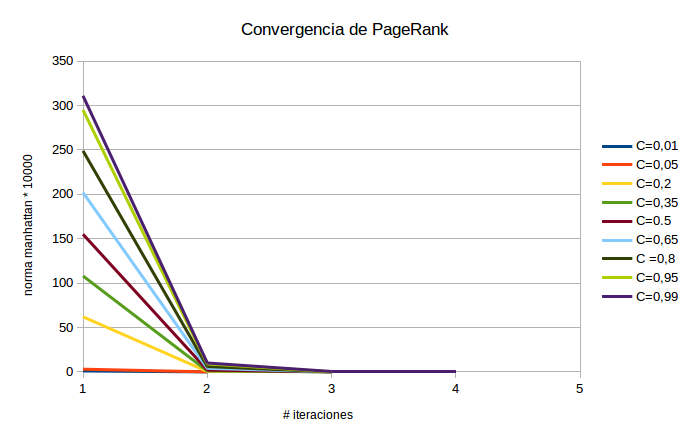
\includegraphics[scale= 0.6]{imagenes/convergencia3.png}
  \end{center}
  \vspace{-20pt}
   \caption{Con tantas páginas y tantos links.}
  \vspace{-10pt}
  \label{fig:img1}
\end{wrapfigure}

Mirando cada gráfico por separado podemos ver que la cantidad de iteraciones del algoritmo disminuye mientras más chico sea el valor de $c$, independientemente de que tan esparsa sea la matriz de links. 
Si comparamos los tres gráficos, vemos que las normas son mas chicas y el algoritmo converge más rápidamente mientras mas completa (menos esparsa) sea la matriz de links.\\



%% FALTA ANALISIS DE POR QUE PASA ESTO %%

%%%%%%%%%%%%%%%%%%%%%%%%%%%%%%%%%%%%%%%%%%%%%%%%%%%%%%%%%%%%%%%%%%%%%%%%%%%%%%%%%%%%%


Para ver como se comporta el algoritmo de $PageRank$ y comparar los resultados con los de $IN-DEG$, proponemos los siguientes ejemplos pequeños. Los grafos representan las páginas web y los link entre ellas, y las tablas muestran los resultados obtenidos de cada algoritmo.\\

%% ACA VAN LAS 6 IMAGENES DE GRAFOS , cada una junto a la tabla de resultados %%

%% ACA EL ANALISIS DE LOS RESULTADOS %%



% \newpage

% \section{Resultados}
A continuación, mostramos los resultados obtenidos de la comparación entre los algoritmos PageRank e IN-DEG para instancias particulares. Dichos resultados son la importancia de cada página j, es decir el $x_{j}$. \\

\begin{figure}[H]
\centering     %%% not \center
\subfigure[Figure A]{\label{fig:a}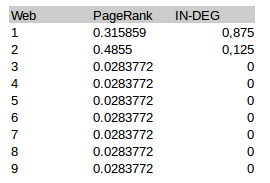
\includegraphics[width=0.4\linewidth]{imagenes/resultadosEstrella.png}}
\subfigure[Figure B]{\label{fig:b}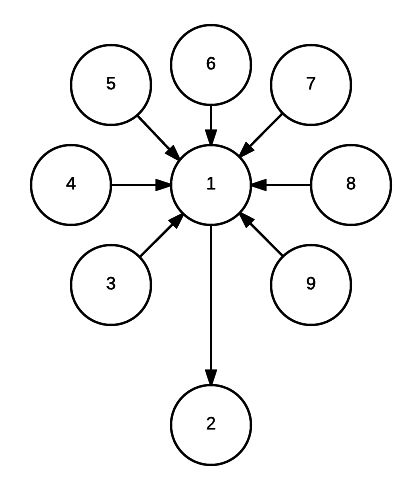
\includegraphics[width=0.3\linewidth]{imagenes/estrella.png}}
\caption{Web con estructura de estrella.}
\end{figure}

En el caso de una web con forma de estrella, cabe destacar las páginas 1 y 2. La página 1 es referenciada por todas las demás, salvo la 2 que es referenciada por la página 1. Dado que IN-DEG definie el ranking de una página j en base a la cantidad de ejes entrantes, es claro que la página uno obtenga la primer posición y la página 2 la segunda posición. Las páginas restantes tienen ranking cero por no ser referenciadas por ninguna otra.
En cambio, para PageRank se hace visible la idea de qué tan importante es el que referencia, en vez de cuantos son los que referencian. Las páginas que no son linkeadas tienen una importancia baja en comparación a las primeras dos.


\begin{figure}[H]
\centering     %%% not \center
\subfigure[Figure A]{\label{fig:a}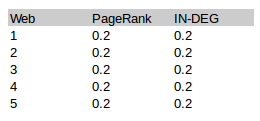
\includegraphics[width=0.4\linewidth]{imagenes/resultadosCompleto.png}}
\subfigure[Figure B]{\label{fig:b}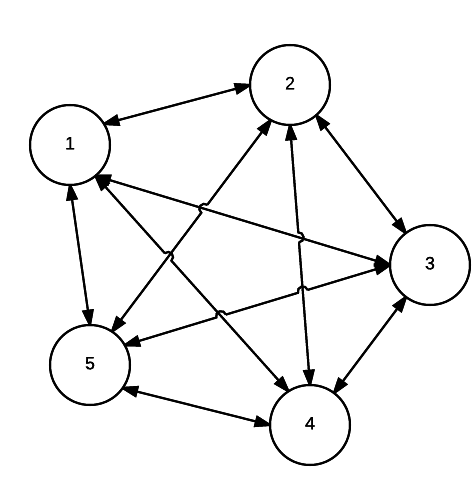
\includegraphics[width=0.3\linewidth]{imagenes/completo.png}}
\caption{Web con estructura de pentágono.}
\end{figure}

El segundo ejemplo, un grafo completo de cinco nodos, lo hicimos para encontrar los casos en que los criterios de importancia de ambos algoritmos coinciden. Era esperable que todas las páginas tengan la misma importancia en ambos dos, ya que todas las páginas web son referenciadas por páginas con la misma importancia.

\begin{figure}[H]
\centering     %%% not \center
\subfigure[Figure A]{\label{fig:a}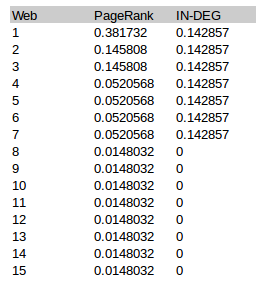
\includegraphics[width=0.3\linewidth]{imagenes/resultadosBinario.png}}
\subfigure[Figure B]{\label{fig:b}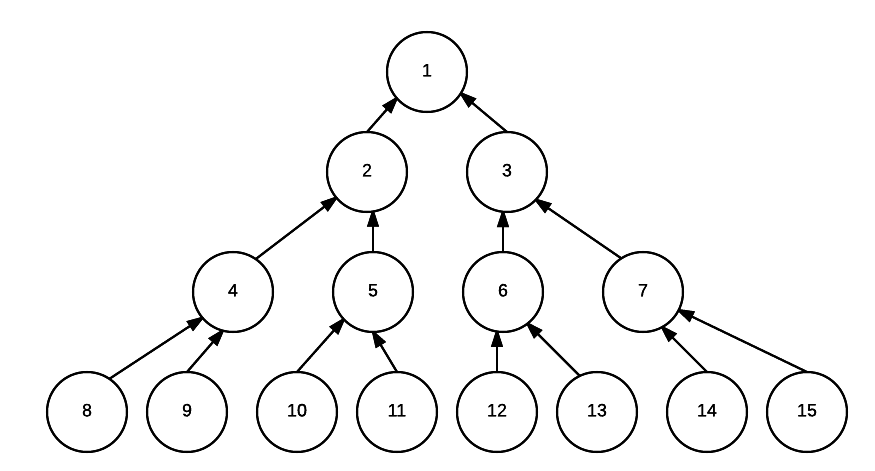
\includegraphics[width=0.5\linewidth]{imagenes/binario.png}}
\caption{my caption}
\end{figure}


\begin{figure}[H]
\centering     %%% not \center
\subfigure[Figure A]{\label{fig:a}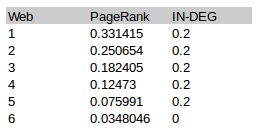
\includegraphics[width=0.4\linewidth]{imagenes/resultadosCamino.png}}
\subfigure[Figure B]{\label{fig:b}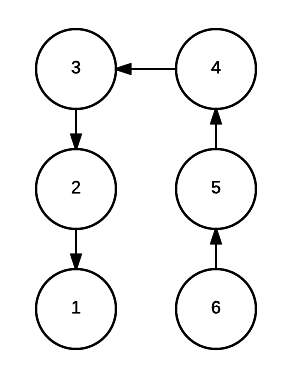
\includegraphics[width=0.2\linewidth]{imagenes/camino.png}}
\caption{my caption}
\end{figure}
% \newpage

% \section{Discusión}
En primer lugar, utilizamos el experimento 1 para poder analizar las variacion de la temperatura para cada angulo del horno. Graficamos los resultados obtenidos para cada radio para observar como se comporta la discipacion del calor en función del radio. De este modo, podriamos entender mejor como se comporta la función para sacar conclusiones de como obtener una mejor aproximacion para encontrar la isoterma pedida.

\begin{figure}[h]
  \center
  \includegraphics[scale=0.8]{imagenes/avanceTemperaturas.png}
  %\caption{La figura}
  \label{fig:avanceTemps}
\end{figure}

Cada curva corresponde a un angulo del horno y se grafica la temperatura para cada radio. Como se puede ver, se corresponden con la familia de funciones $f(x)= \frac{1}{x}$. De este modo, concluimos que utiliazar una regla de tres simple para aproximar la locación de la isoterma no es una aproximación correcta porque guarda una relación lineal, mientras que los datos revelan una relacion inversa multiplicativa. \\
Sin embargo, no resulta una tarea sencilla encontrar una mejor aproxiamción debido a que si la encontraramos, podriamos resolver el problema inicial sin tener que plantear el sistema de ecuaciones planteado anterior. Por tal razón, analizamos alternativas para encontrar una mejor aproximación. Para eso realizamos el experimento 3, para analizar como aumentando el nivel de discretización para una instancia dada, como impacta en el hallazgo de la isoterma. \\
Nuestra hipótesis era que aumentando el nivel de discretización, se refinara la locación de la isoterma, debido a la forma en que la hallamos es encontrar los dos puntos entre los que se encuentra la isoterma. Aumentando la cantidad de puntos, se disminuye la distancia entre los mismos, por lo que el error introducido por la aproximación también debe disminuir. \\
Nos encontramos con un resultado llamativo, que fue darnos cuenta que los primeros puntos no se correspondian con la funcion graficada, y algunos de los primeros puntos tenian un radio menor al radio al que tiende al función. Esto no debería suceder debido a lo siguiente: 
\newpage

\begin{wrapfigure}{l}{0.5\textwidth}
  \vspace{-20pt}
  \begin{center}
    \includegraphics[scale=0.4]{imagenes/aprox.png}
  \end{center}
  \vspace{-20pt}
  \caption{Aproximación lineal contra valor esperado}
  \vspace{-10pt}
  \label{fig:aproximacion}
\end{wrapfigure}

Al utilizar una regla de tres simple, para cada radio obtenido deberíamos obtener un radio ligeramente mayor al radio real de la isoterma, debido a que la función de la discipación del calor tiene una relación inversa multiplicativa.\\
La razón por la que para los primeros valores la función se asemeja a una función lineal, es porque para los primeros casos la isoterma se encuentra entre el radio interno y el siguiente al radio interno. Basamos nuestra aproximación en contar con que el valor de la temperatura hasta el radio $j$ coincide con la función de discipación de calor, y a eso le introducimos un error al aproximar el radio que falta hasta la isoterma. Por lo tanto, si no contamos con valores anteriores al $j$, se cuenta con un error mayor, y la función se asimila más a una lineal que a la que queremos aproximar realmente.\\
Como se ve en la figura \ref{fig:Exp3}, a partir de la instancia en que $m=7$, la función empieza a decrecer y se ve como el valor del radio de la isoterma se estabiliza, debido a que el error se va minimizando por cada nueva división del radio y tiende al valor real del radio de la isoterma. \\

\begin{wrapfigure}{r}{0.5\textwidth}
  \vspace{-20pt}
  \begin{center}
    \includegraphics[scale=0.4]{imagenes/temperaturasInvertidoAmbos.png}
  \end{center}
  \vspace{-20pt}
  \caption{Temperaturas del horno con valores invertidos vs valores normales}
  \vspace{-10pt}
  \label{fig:aproximacion}
\end{wrapfigure}

Por último, el experimento 2, a pesar de ser un caso patológico, no presentó problemas a excepción de que se tuvo que adaptar la función para encontrar la isoterma, dado que no teníamos en cuenta este tipo de casos en un principio. Graficamos las temperaturas de acuerdo al radio para cada punto obtenido, y lo comparamos contra su instancia inversa, es decir, aquella que las temperaturas internas valen 1500 y las externas 0, manteninedo los demás parámetros igual. \\
Lo que sí resultó llamativo, fue hallar que los gráficos son simétricos a partir de la constante 750. Nos encontramos que, si sumamos para cada radio las temperturas de cada instancia, el resultado es siempre 1500. 


% \newpage

% %aca iria apencide
% \section{Conclusiones}

Para este trabajo implementamos algoritmos para rankings tanto de páginas web como de ligas deportivas, dos contextos de aplicación muy distintos para un mismo algoritmo. La implementación de $PageRank$ y de $GeM$ utilizan ambas la misma teoría base y ambas el método de la potencia, por lo que no tuvimos mayor dificultad para implementarlos. Lo que llevó más tiempo fue la implementación de estructuras para matrices que aprovecharan la esparsidad de las mismas y mejoraran el tiempo de ejecución del programa. Esto es importante porque para instancias muy grandes el algoritmo tarda mucho en terminar. Cuando ejecutamos una instancia muy grande con y sin la mejora notamos que es realmente necesario adaptar los programas para que funcionen mejor con los tipos de instancia más comunes que aparecen.

Con respecto a los resultados obtenidos, hicimos comparaciones de rankings generados con los algoritmos de $PageRank$ y $GeM$ y con otros algoritmos más sencillos que usan otros criterios para decidir la importancia de una página (o ranking de un equipo). Notamos muchas diferencias en los resultados con unos u otros algoritmos, pero es difícil decidir cuándo uno es mas justo que otro y podrían tomarse muchisimos criterios distintos para armar un ranking, sobre todo para las páginas web. Para las páginas web podrían entrar muchos otros factores a la hora de ordenar el resultado de la búsqueda. Podría depender, por ejemplo, de quién realiza la búsqueda. Hoy en día es mucho más complejo, pero la base es el método que estudiamos en este trabajo. 

Para los rankings de deportes, estudiamos los resultados generados por $GeM$ en un campeonato real y vimos cómo puede llegar a variar el ranking comparandolo con el método real y otro propuesto por nosotros. Además vimos cómo puede variar cuando modificamos un parámetro del algoritmo de $PageRank$, la probabilidad de teletransportación. En el contexto de una competencia deportiva se puede ver mejor esta variación, no tanto en el contexto de rankings de páginas web.




%la estructura que elegimos





% performance




% la relacion entre la convergencia y el tiempo 




% que nos parecio el trabajo
% \newpage

% \section{Referencias}

\begin{itemize}
\item Burden y J.D.Faires, Análisis numérico, International Thomson Editors, 9na edición
\item Manual de LaTeX: https://es.wikibooks.org/wiki/Manual_de_LaTeX
\item Referencias de C++: http://www.cplusplus.com
\item Referencias de Python: https://docs.python.org/
\end{itemize}
% \newpage

\section{Análisis Espacial de Estructuras de Datos}
\subsection{Propuestas}
Analizamos las distintas alternativas para almacenar la matriz esparsa en términos de eficiencia espacial, comparando en qué casos una alternativa es mejor que otra. Tenemos 4 posibles estructuras de datos para almacenar la matriz. Las opciones propuestas son: \\

\begin{itemize}
	\item \textbf{Vector}: Consiste en almacenar la matriz en un único vector del tamaño de la matriz, almacenando todos los valores de la misma incluyendo los valores nulos.  
	\item \textbf{Dictionary Of Keys (DOK)}: Consiste en almacenar los valores de la matriz que no son nulos en un diccionario, donde las \textit{keys} son la dupla fila y columna, y el \textit{value} es el valor en esa posición. Si una posición no se encuentra en el diccionario, significa que el valor en esa posición es cero.
	\item \textbf{Compressed Sparse Row (CSR)}: Consiste en utilizar 3 \textit{arrays}, uno para guardar todos los valores distintos de cero, otro para guardar la columna donde se encuentran los elementos anteriores, y por último uno donde se almacenan los índices de el primer elemento distinto de cero para cada fila.
	\item \textbf{Compressed Sparse Column (CSC)}: Es igual al CSR, sólo que en lugar de almacenar por filas, se almacena por columnas. El primer \textit{array} guarda los mismos valores pero por columnas, el segundo indica la fila de cada elemento y el último indica el primer elemento distinto de cero de cada columna. La cantidad de memoria que utiliza es exactamente la misma que CSR, dado que los dos primeros $arrays$ tienen igual tamaño (la cantidad de elementos no nulos), y al ser la matriz cuadrada, la cantidad de filas es igual a la de las columnas, coincidiendo así el tamaño del tercer $array$.
\end{itemize}

Para el análisis temporal, optamos por utilizar los valores reales de tamaño que se utiliza en C++, dado que realizando un análsis teórico se llegan a conclusiones que no se corresponden con la implemetación. Un ejemplo sería pensar que una lista de $n$ elementos de tamaño $size\_of\_element$ ocupa un tamaño de $n*size\_of\_element$, cuando en realidad, dependiendo de la implementación, es necesario también tener en cuenta el costo espacial de los punteros para la lista. Si esto no es tenido en cuenta, se podría optar por una estructura de datos que en realidad ocupe más espacio del pensado comparado contra otras alternativas. \\
Para los indices utilizamos el tipo $int$, cuyo tamaño es de 4 bytes, mientras que para los valores almacenados en la matriz utilizamos el tipo $double$ cuyo tamaño es 8 bytes. Para los indices se podría utilizar como alternativa \textit{unsigned int}, que también tienen un tamaño de 4 bytes.\\
Definimos \textbf{NNZ} (NonZero) como la cantidad de valores no nulos de la matriz y $n$ la cantidad de filas (coincidente con las columnas dado que es cuadrada). \\

\subsection{Análisis:}
Para todos los casos, se midió la cantidad de memoria reservada utilizando \textit{valgrind}. Utilizamos para cada caso un pequeño programa que genera una instancia para cada estructura, primero vacía, y luego agregando elementos. De este modo, pudimos observar cuanta memoria utiliza cada estructura por separado. Los resultados del uso de memoria fueron:\\
%http://netlib.org/linalg/html_templates/node91.html

\begin{itemize}
	\item \textbf{Vector}: $n^2 * 8\ bytes$
	\item \textbf{Dictionary Of Keys (DOK)}: $NNZ * 48\ bytes$
	\item \textbf{Compressed Sparse Row (CSR)}: $8*NNZ + 4*NNZ + 4 (n+1)\ bytes$
\end{itemize}

Fue útil tener en cuenta la cantidad de memoria real, principalmente para constatar que tanto Vector como CSR usaran la cantidad teórica estimada, además de saber que DOK utiliza una cantidad mayor a la pensada. Esto se debe a que DOK está implementado sobre el tipo $map$ de C++, que es un Black-Red Tree. Cada elemento cuesta 48 bytes, más que un double ($value$) y dos enteros ($key$), que serían 16 bytes.  \\

Existen casos para los cuales, cada una de las alternativas anteriores es mejor que el resto. Para ejemplificarlo, supongamos que se tiene una matriz con tamaño $n=100$. Graficamos la cantidad de memoria requerida por cada estructura, variando la cantidad de valores distintos de cero: \\ \\

\begin{wrapfigure}{r}{0.6\textwidth}
  \vspace{-20pt}
  \begin{center}
    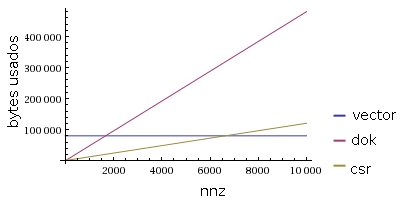
\includegraphics[scale= 0.6]{imagenes/n100espacio.png}
  \end{center}
  \vspace{-20pt}
   \caption[Caption espacio n 100]{Memoria utilizada en una matriz de tamaño 100x100, variando la cantidad de valores no nulos}
  \vspace{-10pt}
  \label{fig:img1}
\end{wrapfigure}

Cabe destacar que, a pesar de no notarse en el gráfico, el Dictionary Of Keys utiliza menos memoria que Compressed Sparse Row para cuando hay menos de 12 valores distintos de cero. A partir de $12 \leq nnz$, Dictionary Of Keys utiliza más memoria. \\ \\ \\ \\  \\
Como conclusión, obtuvimos que Dictionary Of Keys no es una buena implementación en comparación a Compressed Sparse Row en general, a menos que la matriz fuese sumamente esparsa. La relación de la misma se detalla en la siguiente tabla.

\begin{center}
    \begin{tabular}{| l | l | l |}
    \hline
    $n$ & $nnz$ & $nnz/n^2$  \\ \hline
    10	& 1	& \%1 \\ \hline
	100	& 11	& \%0.0011 \\ \hline
	1000 & 111	& \%0.0001 \\ \hline
	5000 & 555 & \%0.00002 \\ \hline
	10000 & 1111 & \%0.000001 \\ \hline
	120000 & 13333 & \%0.00000009 \\ \hline
    \end{tabular}
\end{center}

Los valores $nnz$ son la cantidad de valores no nulos que haría que Dictionary Of Keys utilice menos memoria que Compressed Sparse Row. La relación $nnz/n^2$ muestra el porcentaje de valores no nulos con respecto a la matriz total. Como se observa, la relación debe ser muy baja.\\

Vector es la mejor implemetación para cuando la matriz no es esparsa, en particular cuando se cumple la siguiente desigualdad: $$3 nnz > 2n^2 - n + 1$$

De este modo, para nuestro problema, Compressed Sparse Row presenta la mejor opción en términos espaciales para nuestro problema, con excepción de los casos anteriormente vistos cuando la matriz es sumamente esparsa y cuando muy poco esparsa.
\newpage

\bibliographystyle{plain}
\bibliography{tp3}

\end{document}
